\section{Interpolation}

To analyse an airfoil's surface, a method to model it
with a function was necessary. As the UIUC Applied Aerodynamics Group's airfoil database only gives some pointson the surface, interpolation was needed. There are multiple interpolation
methods like Linear Interpolation or Cubic Spline Interpolation or even some fancier ones, but the selected method had to satisfy two requirements: be continuous and easily derivable.
The Cubic Spline interpolation method was used as it yields a continuous function, is easily derivable without adding algorithmic complexity and 
easy to implement.

\subsection{Cubic Spline Algorithm} \label{Cubic Spline algorithm}
The Cubic Spline approximation can be defined by equation~\ref{eq:cubic_spline_equation},
with $h_i = x_{i+1} - x_i$, $A_i(x) = \frac{x_{i+1}-x}{h_i}$ and $B_i(x) = \frac{x-x_i}{h_i}$:
\begin{equation}
	\label{eq:cubic_spline_equation}
	\begin{split}
		\omega_{\llbracket x_i;x_{i+1} \rrbracket}(x) = &A_i(x)y_i+B_i(x)y_{i+1} \\
		& + \frac{h_i^2}{6}\left(y_i^{''}\left(A_i^3(x) - A_i(x)\right)
		+ y_{i+1}^{''}\left(B_i^3(x) - B_i(x)\right)\right)
	\end{split}
\end{equation}
Each segment from $x_{i}$ to $x_{i+1}$ is interpolated with a cubic polynomial. This allows derivatives up to the second order.

To compute the derivative of a Cubic Spline interpolation, $\omega_i$ has to be derived. Its derivative is defined in equation~\ref{eq:derivative_cubic_spline}:
\begin{equation}
	\label{eq:derivative_cubic_spline}
	\omega_i^{'}(x) = \frac{y_{i+1} - y_i}{h_i} 
		+ \frac{h_i}{6}\left(
			y_i^{''}\left(1-3A_i^2(x)\right)
			+ y_{i+1}^{''}\left(3B_i^2(x)-1\right)
		\right)
\end{equation}

To ensure equation~\ref{eq:derivative_cubic_spline} can be derived, the following condition has to be met: $\forall i \in \llbracket 1;n \rrbracket~\omega_{i-1}^{'}(x_i) = \omega_i^{'}(x_i)$.
This condition can be modelled with equation~\ref{eq:equation_system_cubic_spline}:
\begin{equation}
	\label{eq:equation_system_cubic_spline}
	\frac{h_{i-1}}{6}y_{i-1}^{''} + \frac{h_{i-1} + h_i}{3}y_i^{''} + \frac{h_i}{6}y_{i+1}^{''}
	= \frac{y_{i+1}-y_i}{h_i}-\frac{y_i-y_{i-1}}{h_{i-1}}
\end{equation}
It is essential to specify the value of $y_0^{''}$ and $y_{n+1}^{''}$. For the rest of the experiments, the \textit{natural spline} method was used. It sets both $y_0^{''}$ and $y_{n+1}^{''}$ to $0$.

To get a single function that returns the correct $\omega_i(x)$ for a given $x$ in $\llbracket x_0; x_n \rrbracket$, a function $range(x)$ that searched for the correct range $\llbracket x_i;x_{i+1} \rrbracket$ for a given $x$ was implemented using a binary search algorithm for efficiency's sake as the list of $x_i$ is in increasing order.
Now, the function $\omega(x)$ that gives the interpolation function for all $x$ in $\llbracket x_0;x_n \rrbracket$ is defined as $\omega(x) = \omega_{range(x)}(x)$.

To check whether the Cubic Spline implementation was correctly implemented or not, the results were compared with those from a state of the art library for Cubic Spline interpolation: \verb|scipy|.
The results differed from \verb|scipy|'s one by an order of $10^{-18}$ which was acceptable.

\subsection{Interpolation of the goe05k Airfoil}
An airflow can be separated into 2 surfaces: the extrados (upper curves) and intrados (lower curves).
The database only gives points across both curves as seen in Figure~\ref{fig:sampled_goe05k_airfoil}

Therefore, the Cubic Spline interpolation method was used to model each part of the airfoil as a function to make the analysis of the airfoil possible, as seen in Figure~\ref{fig:interpolated_goe05k_airfoil}.

\begin{figure}[H]
	\centering
	\subfloat[\label{fig:sampled_goe05k_airfoil}\centering The Sampled points of the goe05k airfoil.]{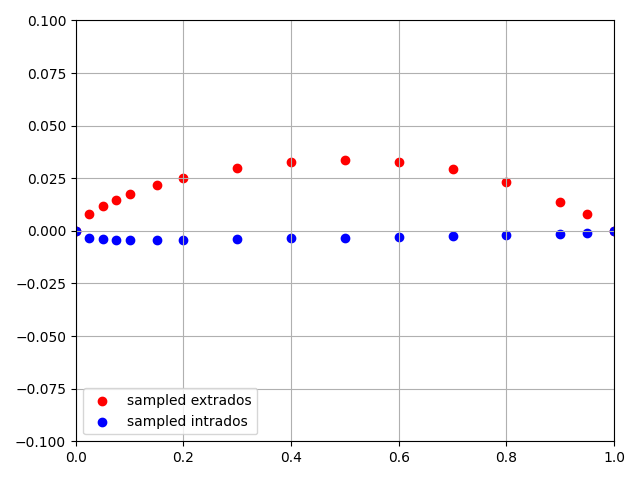
\includegraphics[width=0.45\linewidth]{res/goe05k_sampled.png}}
	\qquad
	\subfloat[\label{fig:interpolated_goe05k_airfoil}\centering The Interpolated goe05k airfoil.]{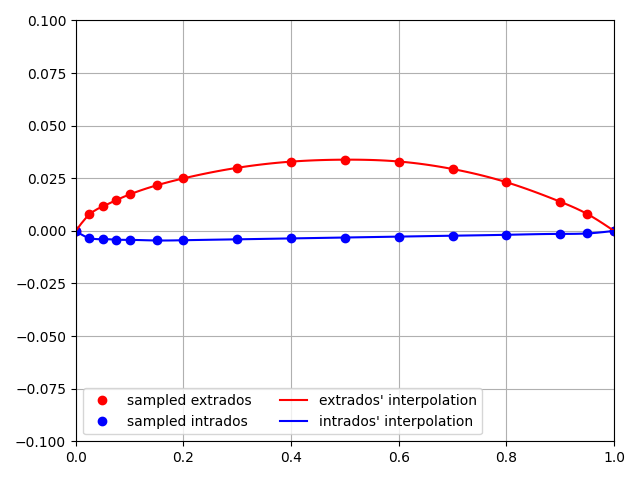
\includegraphics[width=0.45\linewidth]{res/goe05k_interpolated.png}}
	\caption{Interpolation of the goe05k airfoil.}
\end{figure}

\vspace*{-0.7cm}
